% !TEX root = ../sethomas_thesis_main.tex
\documentclass[border=1mm,
               class=article
               preview]{standalone}
\usepackage{tikz}
\begin{document}
\begin{tikzpicture}
    \pgfmathsetmacro{\xLegendA}{1.6}
    \pgfmathsetmacro{\xLegendB}{5.5}
    \pgfmathsetmacro{\xLegendC}{8.98}
    \pgfmathsetmacro{\xLegendD}{12.7}
    \pgfmathsetmacro{\xLegendE}{3.6}
    \pgfmathsetmacro{\xLegendF}{11.1}
    \pgfmathsetmacro{\yLegendBottom}{-0.25}
    \pgfmathsetmacro{\yLegendTop}{2.5}

    % \node[anchor=south west,inner sep=0] (graph) at (0,0){\includegraphics[width=\textwidth]{img/kinematic_schematics_models.pdf}};%kinematic_schematics.pdf
    % \node[anchor=south west,inner sep=0] (graph) at (0,0){\includegraphics[width=\textwidth]{img/kinematic_schematics_models_legend.pdf}};
% 		\node[anchor=south west,inner sep=0] (graph) at (0,0){\includegraphics[width=\textwidth]{img/kinematic_schematics_models_reversed.pdf}};
    \node[anchor=south west,inner sep=0] (graph) at (0,0){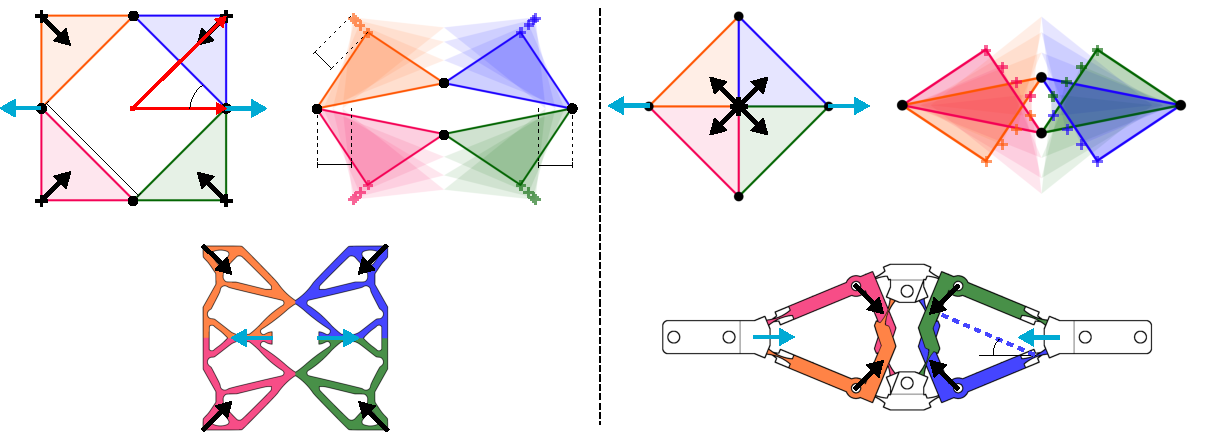
\includegraphics[width=\textwidth]{images/chap7/kinematic_schematics_models_reversed_legend_3.pdf}};
    \coordinate (ts0) at (\xLegendA,\yLegendTop); \node[align=left] at (ts0) {(a)};
    \coordinate (ts1) at (\xLegendB,\yLegendTop); \node[align=left] at (ts1) {(b)};
    \coordinate (ts2) at (\xLegendC,\yLegendTop); \node[align=left] at (ts2) {(c)};
    \coordinate (ts3) at (\xLegendD,\yLegendTop); \node[align=left] at (ts3) {(d)};
    \coordinate (ts4) at (\xLegendE,\yLegendBottom); \node[align=left] at (ts4) {(e)};
    \coordinate (ts5) at (\xLegendF,\yLegendBottom); \node[align=left] at (ts5) {(f)};

    %%%%%%%%%%%%%%%%%%%%%%%%%%%%%%%%%%%%%
    \node[align=left] at (\xLegendA+0.6,\yLegendTop+1.7) {$\theta$};
% 		\node[align=left] at (\xLegendA+0.45,\yLegendTop+2.1) {$\theta$};
% 		\node[align=left] at (\xLegendA+1.8,\yLegendTop+1.) {$L_s$};
    \node[align=left] at (\xLegendA+0.55,\yLegendTop+1.18) {\color{red}$\frac{x}{2}$};
    \node[align=left,rotate=45] at (\xLegendA+0.25,\yLegendTop+2.0) {\small\color{red}$R$};
    \node[align=left,rotate=-44] at (\xLegendA-0.2,\yLegendTop+1.0) {$L_h$};

    \node[align=left] at (\xLegendB+1.3,\yLegendTop+0.4) {$\frac{\Delta x}{2}$};
    \node[align=left] at (\xLegendB-1.5,\yLegendTop+0.4) {$\frac{\Delta x}{2}$};
% 		\node[align=left,rotate=-45] at (\xLegendB-2.1,\yLegendTop+2.35) {\small$R(\Delta x)$};
    \node[align=left,rotate=-45] at (\xLegendB-1.8,\yLegendTop+1.85) {\small$\Delta R$};

    \node[align=left] at (\xLegendF+0.55,\yLegendBottom+1.35) {$\theta_0$};
    % \draw[help lines] (0,0) grid (16,4); % $$$$$$$$$$$$$ HELPS A LOT FOR COORDINATES $$$$$$$
\end{tikzpicture}
\end{document}
